\documentclass[12pt, titlepage]{article}

\usepackage{booktabs}
\usepackage{tabularx}
\usepackage{hyperref}
\hypersetup{
    colorlinks,
    citecolor=black,
    filecolor=black,
    linkcolor=red,
    urlcolor=blue
}
\usepackage[round]{natbib}
\usepackage{geometry}

\usepackage{adjustbox}
\usepackage[dvipsnames]{xcolor}
\usepackage{float}
\usepackage{changepage}
\usepackage{pdflscape}

%% Comments

\usepackage{color}

\newif\ifcomments\commentstrue %displays comments
%\newif\ifcomments\commentsfalse %so that comments do not display

\ifcomments
\newcommand{\authornote}[3]{\textcolor{#1}{[#3 ---#2]}}
\newcommand{\todo}[1]{\textcolor{red}{[TODO: #1]}}
\else
\newcommand{\authornote}[3]{}
\newcommand{\todo}[1]{}
\fi

\newcommand{\wss}[1]{\authornote{blue}{SS}{#1}} 
\newcommand{\plt}[1]{\authornote{magenta}{TPLT}{#1}} %For explanation of the template
\newcommand{\an}[1]{\authornote{cyan}{Author}{#1}}

%% Common Parts

\newcommand{\progname}{Software Engineering} % PUT YOUR PROGRAM NAME HERE
\newcommand{\authname}{Team \#13, ARC
    \\ Avanish, Ahluwalia
    \\ Russell, Davidson
    \\ Rafey, Malik
    \\ Abdul, Zulfiqar} % AUTHOR NAMES                  

\usepackage{hyperref}
    \hypersetup{colorlinks=true, linkcolor=blue, citecolor=blue, filecolor=blue,
                urlcolor=blue, unicode=false}
    \urlstyle{same}
                                


\begin{document}

\title{Verification and Validation Report: \progname}
\author{\authname}
\date{March 10, 2025}

\maketitle

\pagenumbering{roman}

\section{Revision History}

\begin{tabularx}{\textwidth}{p{3cm}p{2cm}X}
  \toprule {\bf Date} & {\bf Version} & {\bf Notes} \\
  \midrule
  2025-03-10              & 1.0           & Initial report\\
  2025-03-28              & 1.1           & Modifications made based on review \\
  \bottomrule
\end{tabularx}

~\newpage

\section{Symbols, Abbreviations and Acronyms}

See SRS Documentation \href{https://github.com/russellrd/realm/blob/main/docs/SRS-IEEE/SRS.pdf}{here} for a full list.\\

\renewcommand{\arraystretch}{1.2}
\begin{tabular}{l l}
  \toprule
  \textbf{symbol} & \textbf{description} \\
  \midrule
  T               & Test                 \\
  \bottomrule
\end{tabular}\\

\newpage

\tableofcontents

\listoftables %if appropriate

\listoffigures %if appropriate

\newpage

\pagenumbering{arabic}

\section{Functional Requirements Evaluation}

\subsection{Database Testing}
The following section presents the results of the our database testing


\begin{table}[H]
  \caption{\bf Functional Requirements Evaluation Results for Database Testing}
  \resizebox{6in}{!}{\begin{tabular}{|l|p{0.15\linewidth}|p{0.3\linewidth}|p{0.3\linewidth}|p{0.3\linewidth}|p{0.1\linewidth}|}
      \hline
      \multicolumn{1}{|l|}{\bfseries Id} & \multicolumn{1}{|l|}{\bfseries Type} & \multicolumn{1}{l|}{\bfseries Inputs}                                      & \multicolumn{1}{l|}{\bfseries Expected Result}                              & \multicolumn{1}{l|}{\bfseries Actual Result} & \multicolumn{1}{l|}{\bfseries Result} \\
      \hline
      Test-DB1                           & Automated                            & Periodic backup run is completed.                                          & Automated monitor verifies that the database backup is present and correct. & Same as expected                             & \textcolor{Green}{Pass}               \\
      \hline
      Test-DB2                           & Automated                            & Command to check encryption status is inputted into DBMS for all databases & DBMS response shows that all databases are encrypted                        & Same as expected                             & \textcolor{Green}{Pass}               \\
      \hline
    \end{tabular}}
  \label{table:GR1}
\end{table}

\subsection{Custom AR Object Generation}
The following section presents the results of our custom AR object generation testing.

\begin{table}[H]
  \caption{\bf Functional Requirements Evaluation Results for Custom AR Object Generation}
  \resizebox{6in}{!}{\begin{tabular}{|l|p{0.15\linewidth}|p{0.3\linewidth}|p{0.3\linewidth}|p{0.3\linewidth}|p{0.1\linewidth}|}
      \hline
      \multicolumn{1}{|l|}{\bfseries Id} & \multicolumn{1}{|l|}{\bfseries Control} & \multicolumn{1}{l|}{\bfseries Inputs}                         & \multicolumn{1}{l|}{\bfseries Expected Result}                                                                     & \multicolumn{1}{l|}{\bfseries Actual Result} & \multicolumn{1}{l|}{\bfseries Result} \\
      \hline
      Test-POG1                          & Automatic                               & Enter prompts of various lengths, with and without profanity. & Prompt is restricted to 200 characters, real-time character count is displayed, profanity is flagged and rejected. & Same as expected                             & \textcolor{Green}{Pass}               \\
      \hline
      Test-POG5                          & Manual                                  & Rotate the AR object to inspect all sides.                    & The AR object rotates smoothly, allowing inspection from all angles.                                               & Same as expected                             & \textcolor{Green}{Pass}               \\
      \hline
    \end{tabular}}
  \label{table:GR2}
\end{table}

\subsection{Uploading Objects to Inventory, Post Object Scan}
The following section presents the results of our testing for uploading objects to inventory after scanning.

\begin{table}[H]
  \caption{\bf Functional Requirements Evaluation Results for Uploading Objects to Inventory}
  \resizebox{6in}{!}{\begin{tabular}{|l|p{0.15\linewidth}|p{0.3\linewidth}|p{0.3\linewidth}|p{0.3\linewidth}|p{0.1\linewidth}|}
      \hline
      \multicolumn{1}{|l|}{\bfseries Id} & \multicolumn{1}{|l|}{\bfseries Control} & \multicolumn{1}{l|}{\bfseries Inputs}                                      & \multicolumn{1}{l|}{\bfseries Expected Result}                                & \multicolumn{1}{l|}{\bfseries Actual Result} & \multicolumn{1}{l|}{\bfseries Result} \\
      \hline
      Test-OUI1                          & Manual                                  & Display the scanned object and allow for user interaction in editing mode. & Render of scanned object is displayed, user can edit and finalize the object. & Same as expected                             & \textcolor{Green}{Pass}               \\
      \hline
      Test-OUI2                          & Manual                                  & Provide a name for the object and save it with metadata.                   & Object name is stored (ASCII only), and all metadata is correctly saved.      & Same as expected                             & \textcolor{Green}{Pass}               \\
      \hline
      Test-OUI3                          & Manual                                  & Select specific portions of the object and apply color changes.            & Color changes are applied accurately and reflected in the final render.       & Same as expected                             & \textcolor{Green}{Pass}               \\
      \hline
    \end{tabular}}
  \label{table:GR3}
\end{table}

\subsection{Realm Testing}
The following section presents the results of our testing of the realm interface.

\begin{table}[H]
  \caption{\bf Functional Requirements Evaluation Results for the Realm Interface}
  \resizebox{6in}{!}{\begin{tabular}{|l|p{0.15\linewidth}|p{0.3\linewidth}|p{0.3\linewidth}|p{0.3\linewidth}|p{0.1\linewidth}|}
      \hline
      \multicolumn{1}{|l|}{\bfseries Id}                                                                           &
      \multicolumn{1}{|l|}{\bfseries Control}                                                                      &
      \multicolumn{1}{l|}{\bfseries Inputs}                                                                        &
      \multicolumn{1}{l|}{\bfseries Expected Result}                                                               &
      \multicolumn{1}{l|}{\bfseries Actual Result}                                                                 &
      \multicolumn{1}{l|}{\bfseries Result}                                                                          \\
      \hline
      Test-RI1                                                                                                     &
      Manual                                                                                                       &
      Tester changes their position and angle in relation to an AR object.                                         &
      The AR object adjusts perspective appropriately, reflecting the new camera position and angle.               &
      Same as expected                                                                                             &
      \textcolor{Green}{Pass}                                                                                        \\
      \hline
      Test-RI2                                                                                                     &
      Manual                                                                                                       &
      Tester moves camera over a crowded area where multiple AR objects are present.                               &
      The interface selectively displays a manageable number of AR objects without overwhelming the user’s view.   &
      Same as expected                                                                                             &
      \textcolor{Green}{Pass}                                                                                        \\
      \hline
      Test-RI3                                                                                                     &
      Manual                                                                                                       &
      Test AR object instance is placed with a known alignment in the real world, and reference screenshots.       &
      Test AR object appears in correct position and orientation as expected, matches stored object instance data. &
      Same as expected                                                                                             &
      \textcolor{Green}{Pass}                                                                                        \\
      \hline
      Test-RI6                                                                                                     &
      Manual                                                                                                       &
      Tester attempts to access the object placement workflow via the provided control.                            &
      Tester is successfully redirected to the object placement workflow.                                          &
      Same as expected                                                                                             &
      \textcolor{Green}{Pass}                                                                                        \\
      \hline
      Test-RI8                                                                                                     &
      Manual                                                                                                       &
      Tester moves within range of the tour start point.                                                           &
      The interface displays a clear indication of the nearby tour and a link to the tour preview.                 &
      Same as expected                                                                                             &
      \textcolor{Green}{Pass}                                                                                        \\
      \hline
      Test-RI9                                                                                                     &
      Manual                                                                                                       &
      Tester moves closer to a hazard in real space.                                                               &
      Interface displays a clear warning when the user approaches the hazard.                                      &
      Same as expected                                                                                             &
      \textcolor{Green}{Pass}                                                                                        \\
      \hline
    \end{tabular}}
  \label{table:Realm_Interface_Tests}
\end{table}

\subsection{Object Placement Testing}
The following section presents the results of our object placement testing.

\begin{table}[H]
  \caption{\bf Functional Requirements Evaluation Results for Object Placement Features}
  \resizebox{6in}{!}{\begin{tabular}{|l|p{0.15\linewidth}|p{0.3\linewidth}|p{0.3\linewidth}|p{0.3\linewidth}|p{0.1\linewidth}|}
      \hline
      \multicolumn{1}{|l|}{\bfseries Id}                                                                   &
      \multicolumn{1}{|l|}{\bfseries Control}                                                              &
      \multicolumn{1}{l|}{\bfseries Inputs}                                                                &
      \multicolumn{1}{l|}{\bfseries Expected Result}                                                       &
      \multicolumn{1}{l|}{\bfseries Actual Result}                                                         &
      \multicolumn{1}{l|}{\bfseries Result}                                                                  \\
      \hline
      Test-OP1                                                                                             &
      Manual                                                                                               &
      Tester selects object from inventory or prompt generation.                                           &
      Interface successfully proceeds to the placement interface with the selected object.                 &
      Same as expected                                                                                     &
      \textcolor{Green}{Pass}                                                                                \\
      \hline
      Test-OP3                                                                                             &
      Manual                                                                                               &
      Tester rotates, resizes, and translates the object in real space.                                    &
      Object is placed accurately in real space with correct orientation.                                  &
      Same as expected                                                                                     &
      \textcolor{Green}{Pass}                                                                                \\
      \hline
      Test-OP4                                                                                             &
      Manual                                                                                               &
      Tester checks the AR object instance database.                                                       &
      Object instance is present with correct details (type, position, orientation).                       &
      Same as expected                                                                                     &
      \textcolor{Green}{Pass}                                                                                \\
      \hline
      Test-OP5                                                                                             &
      Automated and Manual                                                                                 &
      Tester attempts to place another object in an area with placement limit reached.                     &
      System prevents additional placements, displaying a warning.                                         &
      Same as expected                                                                                     &
      \textcolor{Green}{Pass}                                                                                \\
      \hline
      Test-OP6                                                                                             &
      Automated and Manual                                                                                 &
      Tester attempts to place another object within a short period after the time-based limit is reached. &
      System restricts further placements, displaying a warning.                                           &
      Same as expected                                                                                     &
      \textcolor{Green}{Pass}                                                                                \\
      \hline
      Test-OP7                                                                                             &
      Automated and Manual                                                                                 &
      Tester places an object, but the initial storage attempt fails.                                      &
      System automatically retries storage until success or retry limit is reached.                        &
      Same as expected                                                                                     &
      \textcolor{Green}{Pass}                                                                                \\
      \hline
    \end{tabular}}
  \label{table:Object_Placement_Tests}
\end{table}


\subsection{Interactions with User Inventory}
The following section presents the results of our testing of interactions with the user inventory.

\begin{table}[H]
  \caption{\bf Functional Requirements Evaluation Results for Inventory Features}
  \resizebox{6in}{!}{\begin{tabular}{|l|p{0.15\linewidth}|p{0.3\linewidth}|p{0.3\linewidth}|p{0.3\linewidth}|p{0.1\linewidth}|}
      \hline
      \multicolumn{1}{|l|}{\bfseries Id}                                       &
      \multicolumn{1}{|l|}{\bfseries Control}                                  &
      \multicolumn{1}{l|}{\bfseries Inputs}                                    &
      \multicolumn{1}{l|}{\bfseries Expected Result}                           &
      \multicolumn{1}{l|}{\bfseries Actual Result}                             &
      \multicolumn{1}{l|}{\bfseries Result}                                      \\
      \hline
      Test-IV1                                                                 &
      Manual                                                                   &
      Tester selects an object and chooses the delete option.                  &
      The selected object is removed from the inventory.                       &
      Same as expected                                                         &
      \textcolor{Green}{Pass}                                                    \\
      \hline
      Test-IV2                                                                 &
      Manual                                                                   &
      Tester adds a new object to the inventory.                               &
      The new object appears in the inventory.                                 &
      Same as expected                                                         &
      \textcolor{Green}{Pass}                                                    \\
      \hline
      Test-IV3                                                                 &
      Automatic                                                                &
      Tester opens the inventory.                                              &
      Inventory contains the preloaded application-provided objects.           &
      Same as expected                                                         &
      \textcolor{Green}{Pass}                                                    \\
      \hline
      Test-IV4                                                                 &
      Automatic                                                                &
      Tester attempts to add an additional object.                             &
      The object is successfully added, but adding another would be prevented. &
      Same as expected                                                         &
      \textcolor{Green}{Pass}                                                    \\
      \hline
      Test-IV5                                                                 &
      Manual                                                                   &
      Tester opens the inventory and inspects object origins.                  &
      Each personal object is present.                                         &
      Same as expected                                                         &
      \textcolor{Green}{Pass}                                                    \\
      \hline
      Test-IV6                                                                 &
      Automatic                                                                &
      Tester views the total count of objects.                                 &
      The app displays the correct total number of objects.                    &
      Same as expected                                                         &
      \textcolor{Green}{Pass}                                                    \\
      \hline
      Test-IV7                                                                 &
      Manual                                                                   &
      Tester adds both 2D and 3D AR objects to their inventory.                &
      Both 2D and 3D objects are correctly stored in inventory.                &
      Same as expected                                                         &
      \textcolor{Green}{Pass}                                                    \\
      \hline
      Test-IV9                                                                 &
      Manual                                                                   &
      Tester sorts objects by usage or size.                                   &
      Objects are sorted as per user selection.                                &
      Same as expected                                                         &
      \textcolor{Green}{Pass}                                                    \\
      \hline
      Test-IV10                                                                &
      Automatic                                                                &
      Tester selects option to view a 3D AR object.                            &
      3D objects are displayed in a continuous rotating state.                 &
      Same as expected                                                         &
      \textcolor{Green}{Pass}                                                    \\
      \hline
    \end{tabular}}
  \label{table:Inventory_Tests}
\end{table}
\subsection{Profile Testing}
The following section presents the results of the profile testing


\begin{table}[H]
  \caption{\bf Functional Requirements Evaluation Results for Profile Testing}
  \resizebox{6in}{!}{\begin{tabular}{|l|p{0.15\linewidth}|p{0.3\linewidth}|p{0.3\linewidth}|p{0.3\linewidth}|p{0.1\linewidth}|}
      \hline
      \multicolumn{1}{|l|}{\bfseries Id} & \multicolumn{1}{|l|}{\bfseries Type} & \multicolumn{1}{l|}{\bfseries Inputs}                                      & \multicolumn{1}{l|}{\bfseries Expected Result}                              & \multicolumn{1}{l|}{\bfseries Actual Result} & \multicolumn{1}{l|}{\bfseries Result} \\
      \hline
      Test-PS1                           & Manual                            & User enters valid credentials.                                          &  The user successfully logs in and
is redirected to their profile page. & Same as expected                             & \textcolor{Green}{Pass}               \\
      \hline
      Test-PS2                           & Manual                            & User inputs new password and confirms. & System updates the password
and provides a confirmation message.                        & Same as expected                             & \textcolor{Green}{Pass}               \\
      \hline
    Test-PS3                           & Automated                            & None & Profile information (username,
password, status) is displayed correctly.                        & Same as expected                             & \textcolor{Green}{Pass}               \\
      \hline
    Test-PS4                           & Manual                            & User navigates to help page. & A help page with FAQs and ad-
ditional help information is displayed.                        & Same as expected                             & \textcolor{Green}{Pass}               \\
      \hline
    \end{tabular}}
\label{table:GR7}
\end{table}

\subsection{Touring}
The following section presents the results of the general users experience of using a tour.


\begin{table}[H]
  \caption{\bf Functional Requirements Evaluation Results for Touring}
  \resizebox{6in}{!}{\begin{tabular}{|l|p{0.15\linewidth}|p{0.3\linewidth}|p{0.3\linewidth}|p{0.3\linewidth}|p{0.1\linewidth}|}
      \hline
      \multicolumn{1}{|l|}{\bfseries Id} & \multicolumn{1}{|l|}{\bfseries Type} & \multicolumn{1}{l|}{\bfseries Inputs}                                      & \multicolumn{1}{l|}{\bfseries Expected Result}                              & \multicolumn{1}{l|}{\bfseries Actual Result} & \multicolumn{1}{l|}{\bfseries Result} \\
      \hline
      Test-TR1                           & Manual                            & General user attempts to navigate to the touring screen.                                          &  The touring screen is reachable. & Same as expected                             & \textcolor{Green}{Pass}               \\
      \hline
      Test-TR2                           & Manual                            & Organization user attempts to navigate to touring screen. & The touring screen is hidden from user.                        & Same as expected                             & \textcolor{Green}{Pass}               \\
      \hline
    Test-TR3                           & Manual                            & General user finds a tour and attempts to preview it & User can see the information described in TR-FR3.                        & Same as expected                             & \textcolor{Green}{Pass}               \\
      \hline
    Test-TR4                           & Manual                            & General user navigates to the tour list interface, and searches for a tour
belonging to an organization. & The tour has been found.                      & Same as expected                             & \textcolor{Green}{Pass}               \\
      \hline
    Test-TR5                           & Manual                            & General user goes close to a tour area in the real-world & A push notification appears on the user’s phone indicating
that a tour is nearby and prompts them to preview it.                      & Same as expected                             & \textcolor{Green}{Pass}               \\
        \hline
      Test-TR6                           & Manual                            & General user scans the QR code through the camera app. & The camera app opens Realm to the preview of the corre-
sponding tour.                        & Same as expected                             & \textcolor{Green}{Pass}               \\
      \hline
      Test-TR8                           & Manual                            & General user selects map view & The user can see the map with the properties described in
TR-FR4.1.                        & Same as expected                             & \textcolor{Green}{Pass}               \\
      \hline
    \end{tabular}}
\label{table:GR6}
\end{table}

\subsection{Tour management}
The following section presents the results of the organizational users side of managing a tour.

\begin{table}[H]
  \caption{\bf Functional Requirements Evaluation Results for Managing Tours}
  \resizebox{6in}{!}{\begin{tabular}{|l|p{0.15\linewidth}|p{0.3\linewidth}|p{0.3\linewidth}|p{0.3\linewidth}|p{0.1\linewidth}|}
      \hline
      \multicolumn{1}{|l|}{\bfseries Id} & \multicolumn{1}{|l|}{\bfseries Control} & \multicolumn{1}{l|}{\bfseries Inputs}                                      & \multicolumn{1}{l|}{\bfseries Expected Result}                                & \multicolumn{1}{l|}{\bfseries Actual Result} & \multicolumn{1}{l|}{\bfseries Result} \\
      \hline
       Test-TM1                           & Manual                            & Organization user attempts to navigate to tour management screen.                                          &  The tour management screen is reachable. & Same as expected                             & \textcolor{Green}{Pass}               \\
      \hline
      Test-TM2                           & Manual                            & General user attempts to navigate to tour management screen. & The tour management screen is hidden from user.                        & Same as expected                             & \textcolor{Green}{Pass}               \\
      \hline
    Test-TM3                           & Manual                            & User attempts to create a tour by inputting all the information
described in TM-FR4 and placing one of each type of object in the
environment. & The tour is successfully created with the correct data.                        & Same as expected                             & \textcolor{Green}{Pass}               \\
      \hline
    Test-TM4                           & Manual                            & User attempts to create a tour by inputting all the information
described in TM-FR4 and selects the option to save as a draft. & The tour is successfully created as a draft.                     & Tours aren't being saved as a draft                             & \textcolor{Red}{Fail}               \\
      \hline
    Test-TM5                           & Manual                            & Organization user attempts to create a tour by inputting all the information
described in TM-FR4 and selects the option to publish the tour. & The tour is successfully created and published.                      & Same as expected                             & \textcolor{Green}{Pass}               \\
        \hline
      Test-TM6                           & Manual                            & User navigates to the draft tour and selects publish option. & The tour is successfully published.                        & Draft not published since tours aren't being saved as a draft.                               & \textcolor{Red}{Fail}               \\
      \hline
    Test-TM7                           & Manual                            & User navigates to the tour and selects the preview option. & The tour can be previewed through the lens of what a Gen-
eral User would see.                        & Same as expected                             & \textcolor{Green}{Pass}               \\
      \hline
      Test-TM8                           & Manual                            & User navigates to the tour they wish to edit, selects the edit
option and changes all the inputs described in TM-FR4. & The tour is successfully edited with the correct data.                     & Same as expected                             & \textcolor{Green}{Pass}               \\
      \hline
    \end{tabular}}
  \label{table:GR5}
\end{table}

\restoregeometry
\section{Nonfunctional Requirements Evaluation}

\subsection{Usability Testing}
The following section presents the results of our usability testing.

\begin{table}[H]
  \caption{\bf Usability Testing Evaluation Results}
  \resizebox{6in}{!}{\begin{tabular}{|l|p{0.15\linewidth}|p{0.3\linewidth}|p{0.3\linewidth}|p{0.3\linewidth}|p{0.1\linewidth}|}
      \hline
      \multicolumn{1}{|l|}{\bfseries Id} & \multicolumn{1}{|l|}{\bfseries Type} & \multicolumn{1}{l|}{\bfseries Inputs}                                         & \multicolumn{1}{l|}{\bfseries Expected Result}                                   & \multicolumn{1}{l|}{\bfseries Actual Result} & \multicolumn{1}{l|}{\bfseries Result} \\
      \hline
      Test-QS-U1                         & Manual                               & Language setting is changed to English, Mandarin, Hindi, Spanish, and French. & Text updates correctly in all tested languages with understandable translations. & Same as expected                             & \textcolor{Green}{Pass}               \\
      \hline
      Test-QS-U2                         & Manual                               & New users perform core app workflows without guidance.                        & 80\% of testers complete tasks and rate the app as intuitive and satisfying.     & Same as expected                             & \textcolor{Green}{Pass}               \\
      \hline
    \end{tabular}}
  \label{table:GR-Usability}
\end{table}

\subsection{Security Testing}
The following section presents the results of our security testing.

\begin{table}[H]
  \caption{\bf Security Testing Evaluation Results}
  \resizebox{6in}{!}{\begin{tabular}{|l|p{0.15\linewidth}|p{0.3\linewidth}|p{0.3\linewidth}|p{0.3\linewidth}|p{0.1\linewidth}|}
      \hline
      \multicolumn{1}{|l|}{\bfseries Id} & \multicolumn{1}{|l|}{\bfseries Type} & \multicolumn{1}{l|}{\bfseries Inputs}                                        & \multicolumn{1}{l|}{\bfseries Expected Result}     & \multicolumn{1}{l|}{\bfseries Actual Result} & \multicolumn{1}{l|}{\bfseries Result} \\
      \hline
      Test-QS-SC3                        & Manual                               & Code sections displaying private data are checked for identity verification. & All sections contain identity verification checks. & Same as expected                             & \textcolor{Green}{Pass}               \\
      \hline
    \end{tabular}}
  \label{table:GR-Security}
\end{table}

\subsection{Availability Testing}
The following section presents the results of our availability testing.

\begin{table}[H]
  \caption{\bf Availability Testing Evaluation Results}
  \resizebox{6in}{!}{\begin{tabular}{|l|p{0.15\linewidth}|p{0.3\linewidth}|p{0.3\linewidth}|p{0.3\linewidth}|p{0.1\linewidth}|}
      \hline
      \multicolumn{1}{|l|}{\bfseries Id} & \multicolumn{1}{|l|}{\bfseries Type} & \multicolumn{1}{l|}{\bfseries Inputs} & \multicolumn{1}{l|}{\bfseries Expected Result} & \multicolumn{1}{l|}{\bfseries Actual Result} & \multicolumn{1}{l|}{\bfseries Result} \\
      \hline
      Test-QS-A1                         & Automated                            & Monitor server uptime over one week.  & Server uptime recorded at 99\% or higher.      & Same as expected                             & \textcolor{Green}{Pass}               \\
      \hline
    \end{tabular}}
  \label{table:GR-Availability}
\end{table}

\subsection{Maintainability Testing}
The following section presents the results of our maintainability testing.

\begin{table}[H]
  \caption{\bf Maintainability Testing Evaluation Results}
  \resizebox{6in}{!}{\begin{tabular}{|l|p{0.15\linewidth}|p{0.3\linewidth}|p{0.3\linewidth}|p{0.3\linewidth}|p{0.1\linewidth}|}
      \hline
      \multicolumn{1}{|l|}{\bfseries Id}                                                                             &
      \multicolumn{1}{|l|}{\bfseries Control}                                                                        &
      \multicolumn{1}{l|}{\bfseries Inputs}                                                                          &
      \multicolumn{1}{l|}{\bfseries Expected Result}                                                                 &
      \multicolumn{1}{l|}{\bfseries Actual Result}                                                                   &
      \multicolumn{1}{l|}{\bfseries Result}                                                                            \\
      \hline
      Test-DI-M1                                                                                                     &
      Manual and Automated                                                                                           &
      Simulate common errors like database connection failure, invalid input data, service timeout in internal APIs. &
      Error messages clearly indicate the source and nature of the error (90\% of the cases).                        &
      Same as expected                                                                                               &
      \textcolor{Green}{Pass}                                                                                          \\
      \hline
    \end{tabular}}
  \label{table:Maintainability_Tests}
\end{table}

\subsection{Compliance Testing}
The following section presents the results of our compliance testing.

\begin{table}[H]
  \caption{\bf Compliance Testing Evaluation Results}
  \resizebox{6in}{!}{\begin{tabular}{|l|p{0.15\linewidth}|p{0.3\linewidth}|p{0.3\linewidth}|p{0.3\linewidth}|p{0.1\linewidth}|}
      \hline
      \multicolumn{1}{|l|}{\bfseries Id}                                                            &
      \multicolumn{1}{|l|}{\bfseries Control}                                                       &
      \multicolumn{1}{l|}{\bfseries Inputs}                                                         &
      \multicolumn{1}{l|}{\bfseries Expected Result}                                                &
      \multicolumn{1}{l|}{\bfseries Actual Result}                                                  &
      \multicolumn{1}{l|}{\bfseries Result}                                                           \\
      \hline
      Test-CO1                                                                                      &
      Manual                                                                                        &
      App is checked against the Personal Information and Electronic Documents Act (PIPEDA).        &
      The app complies with all sections of PIPEDA.                                                 &
      Same as expected                                                                              &
      \textcolor{Green}{Pass}                                                                         \\
      \hline
      Test-CO2                                                                                      &
      Manual                                                                                        &
      The app's revenue records are checked for purchases and ad-revenue spanning at least 6 years. &
      The records go back at least 6 years.                                                         &
      N/A                                                                                           &
      \\
      \hline
      Test-CO3                                                                                      &
      Manual                                                                                        &
      App is checked against the Google Play Developer Policy.                                      &
      The app complies with all sections of the Google Play Developer Policy.                       &
      Same as expected                                                                              &
      \textcolor{Green}{Pass}                                                                         \\
      \hline
      Test-CO4                                                                                      &
      Manual                                                                                        &
      App is checked against the App Store Review Guidelines.                                       &
      The app complies with all sections of the App Store Review Guidelines.                        &
      Same as expected                                                                              &
      \textcolor{Green}{Pass}                                                                         \\
      \hline
    \end{tabular}}
  \label{table:Compliance_Tests}
\end{table}

\subsection{Reusability Testing}
The following section presents the results of our reusability testing.

\begin{table}[H]
  \caption{\bf Reusability Testing Evaluation Results}
  \resizebox{6in}{!}{\begin{tabular}{|l|p{0.15\linewidth}|p{0.3\linewidth}|p{0.3\linewidth}|p{0.3\linewidth}|p{0.1\linewidth}|}
      \hline
      \multicolumn{1}{|l|}{\bfseries Id}                                                                                       &
      \multicolumn{1}{|l|}{\bfseries Control}                                                                                  &
      \multicolumn{1}{l|}{\bfseries Inputs}                                                                                    &
      \multicolumn{1}{l|}{\bfseries Expected Result}                                                                           &
      \multicolumn{1}{l|}{\bfseries Actual Result}                                                                             &
      \multicolumn{1}{l|}{\bfseries Result}                                                                                      \\
      \hline
      Test-DI-R1                                                                                                               &
      Static                                                                                                                   &
      All code is sent to a static analyzer that detects code duplication.                                                     &
      The analysis shows metrics related to code sections with a high amount of duplication, suggesting areas for refactoring. &
      Some duplicate code was found. Refactoring to fix this issue.                                                            &
      \textcolor{Red}{Fail}                                                                                                      \\
      \hline
    \end{tabular}}
  \label{table:Reusability_Tests}
\end{table}

\subsection{Maps Interface Testing}
The following table presents the results of the our maps interface testing:

\begin{table}[H]
  \caption{\bf Functional Requirements Evaluation Results for Maps Interface Testing}
  \resizebox{6in}{!}{\begin{tabular}{|l|p{0.15\linewidth}|p{0.3\linewidth}|p{0.3\linewidth}|p{0.3\linewidth}|p{0.1\linewidth}|}
      \hline
      \multicolumn{1}{|l|}{\bfseries Id} & \multicolumn{1}{|l|}{\bfseries Type} & \multicolumn{1}{l|}{\bfseries Inputs}                                                                   & \multicolumn{1}{l|}{\bfseries Expected Result}                                                                                                                                                                                                                                         & \multicolumn{1}{l|}{\bfseries Actual Result} & \multicolumn{1}{l|}{\bfseries Result} \\
      \hline
      Test-MP1                           & Manual                               & Tester is present on the Map interface and is viewing the complete map and check displayed information. & \begin{enumerate} \item User's current location is displayed on the map. \item Location markers appear for AR object clusters. \item Markers show the count of objects in each cluster. \item All sub-realm objects associated with the user are indicated on the map. \end{enumerate} & Same as expected                             & \textcolor{Green}{Pass}               \\
      \hline
      Test-MP2                           & Manual                               & Select a marker and initiate navigation. Terminate navigation mid-route.                                & \begin{enumerate} \item Directions to the selected marker are provided. \item Navigation terminates when requested by the user. \end{enumerate}                                                                                                                                        & Same as expected                             & \textcolor{Green}{Pass}               \\
      \hline
      Test-MP3                           & Automated                            & Zoom in and out on the map and navigate toward restricted areas.                                        & \begin{enumerate} \item Objects are grouped to reduce clutter on the map. \item Restricted areas are identified, and navigation to these areas is disallowed. \end{enumerate}                                                                                                          & Same as expected                             & \textcolor{Green}{Pass}               \\
      \hline
    \end{tabular}}
  \label{table:MP}
\end{table}

\subsection{Settings Testing}
The following table presents the results of the our settings testing:

\begin{table}[H]
  \caption{\bf Functional Requirements Evaluation Results for Settings Testing}
  \resizebox{6in}{!}{\begin{tabular}{|l|p{0.15\linewidth}|p{0.3\linewidth}|p{0.3\linewidth}|p{0.3\linewidth}|p{0.1\linewidth}|}
      \hline
      \multicolumn{1}{|l|}{\bfseries Id} & \multicolumn{1}{|l|}{\bfseries Type} & \multicolumn{1}{l|}{\bfseries Inputs}                                                               & \multicolumn{1}{l|}{\bfseries Expected Result}                                      & \multicolumn{1}{l|}{\bfseries Actual Result} & \multicolumn{1}{l|}{\bfseries Result} \\
      \hline
      Test-S1                            & Manual                               & User adjusts text size, enables/disables viewing of object names, or changes language.              & The expected result is that accessibility settings apply as configured by the user. & Same as expected                             & \textcolor{Green}{Pass}               \\
      \hline
      Test-S2                            & Manual                               & User changes display settings such as light/dark mode or AR object visibility.                      & The expected result is that display settings reflect user preferences.              & Same as expected                             & \textcolor{Green}{Pass}               \\
      \hline
      Test-S3                            & Manual                               & User modifies privacy settings to control visibility of profile, friends list, and AR interactions. & The expected result is that privacy settings update based on user preferences.      & Same as expected                             & \textcolor{Green}{Pass}               \\
      \hline
      Test-S4                            & Manual                               & User changes username, password, profile picture, or status.                                        & The expected result is that profile settings are updated and saved.                 & Same as expected                             & \textcolor{Green}{Pass}               \\
      \hline
      Test-S5                            & Manual                               & User navigates to sub-realm settings to modify sub-realm options.                                   & The expected result is that sub-realm settings are accessible and configurable.     & Same as expected                             & \textcolor{Green}{Pass}               \\
      \hline
    \end{tabular}}
  \label{table:ST}
\end{table}

\subsection{Portability Testing}
The following table presents the results of the portability testing:

\begin{table}[H]
  \caption{\bf Portability Testing Evaluation Results}
  \resizebox{6in}{!}{\begin{tabular}{|l|p{0.15\linewidth}|p{0.3\linewidth}|p{0.3\linewidth}|p{0.3\linewidth}|p{0.1\linewidth}|}
      \hline
      \multicolumn{1}{|l|}{\bfseries Id} & \multicolumn{1}{|l|}{\bfseries Type} & \multicolumn{1}{l|}{\bfseries Inputs}                                                                      & \multicolumn{1}{l|}{\bfseries Expected Result}                               & \multicolumn{1}{l|}{\bfseries Actual Result} & \multicolumn{1}{l|}{\bfseries Result} \\
      \hline
      Test-PT1                           & Non-Functional, Manual               & Run the app on iOS and Android devices.                                                                    & The app is functional and displays correctly on both platforms.              & App works correctly on both devices          & \textcolor{Green}{Pass}               \\
      \hline
      Test-PT2                           & Non-Functional, Code Review          & Inspect the codebase to ensure shared files are correctly configured with minimal platform-specific files. & Codebase only differs in configuration files for platform-specific settings. & Same as expected                             & \textcolor{Green}{Pass}               \\
      \hline
      Test-PT3                           & Non-Functional, Automated            & Initiate automated builds for both iOS and Android.                                                        & Both builds succeed without errors.                                          & Same as expected                             & \textcolor{Green}{Pass}               \\
      \hline
    \end{tabular}}
  \label{table:NFR-Portability}
\end{table}

\subsection{Safety Testing}
The following table presents the results of the safety testing:

\begin{table}[H]
  \caption{\bf Safety Testing Evaluation Results}
  \resizebox{6in}{!}{\begin{tabular}{|l|p{0.15\linewidth}|p{0.3\linewidth}|p{0.3\linewidth}|p{0.3\linewidth}|p{0.1\linewidth}|}
      \hline
      \multicolumn{1}{|l|}{\bfseries Id} & \multicolumn{1}{|l|}{\bfseries Type} & \multicolumn{1}{l|}{\bfseries Inputs}                                              & \multicolumn{1}{l|}{\bfseries Expected Result}                                                                          & \multicolumn{1}{l|}{\bfseries Actual Result}                                                                         & \multicolumn{1}{l|}{\bfseries Result} \\
      \hline
      Test-SA1                           & Non-Functional, Survey-Based         & Conduct a user survey after users engage with the app in a controlled environment. & Survey results show that users do not find the app dangerously distracting them from their surroundings while using it. & Based on the survey results shown in the \hyperref[table:US1]{table} below, users find the app somewhat distracting. & \textcolor{Red}{Fail}                 \\
      \hline
      Test-SA2                           & Non-Functional, Manual Inspection    & Navigate through all screens and interactions within the app.                      & No bright flashes or loud noises are present in any of the app interfaces.                                              & No bright flashes were noticed. Loud Noises are not heard on any user interface.                                     & \textcolor{Green}{Pass}               \\
      \hline
    \end{tabular}}
  \label{table:NFR-Safety}
\end{table}

\subsection{Installation Testing}
The following table presents the results of the installation testing:

\begin{table}[H]
  \caption{\bf Installation Testing Evaluation Results}
  \resizebox{6in}{!}{\begin{tabular}{|l|p{0.15\linewidth}|p{0.3\linewidth}|p{0.3\linewidth}|p{0.3\linewidth}|p{0.1\linewidth}|}
      \hline
      \multicolumn{1}{|l|}{\bfseries Id} & \multicolumn{1}{|l|}{\bfseries Type} & \multicolumn{1}{l|}{\bfseries Inputs}                                                       & \multicolumn{1}{l|}{\bfseries Expected Result}                            & \multicolumn{1}{l|}{\bfseries Actual Result} & \multicolumn{1}{l|}{\bfseries Result} \\
      \hline
      Test-I1                            & Non-Functional, Manual               & Search for the app on the Apple App Store and Google Play Store.                            & The app is available for download on both app stores.                     & Same as expected                             & \textcolor{Green}{Pass}               \\
      \hline
      Test-I2                            & Non-Functional, Manual               & Attempt to install the app on a device from both the Apple App Store and Google Play Store. & The app installs directly without any additional steps or configurations. & Same as expected                             & \textcolor{Green}{Pass}               \\
      \hline
    \end{tabular}}
  \label{table:NFR-Installation}
\end{table}

\subsection{Performance Testing}
The following section presents the results of our performance testing.

\begin{table}[H]
  \caption{\bf Performance Testing Evaluation Results}
  \resizebox{6in}{!}{\begin{tabular}{|l|p{0.15\linewidth}|p{0.3\linewidth}|p{0.3\linewidth}|p{0.3\linewidth}|p{0.1\linewidth}|}
      \hline
      \multicolumn{1}{|l|}{\bfseries Id} & \multicolumn{1}{|l|}{\bfseries Type} & \multicolumn{1}{l|}{\bfseries Inputs}                                         & \multicolumn{1}{l|}{\bfseries Expected Result}                                   & \multicolumn{1}{l|}{\bfseries Actual Result} & \multicolumn{1}{l|}{\bfseries Result} \\
      \hline
      Test-QS-PE1                         & Automatic                               & User performs actions to navigate to the Map in-
terface. & The map and its overlays are completely visible and
can be interacted with. & Same as expected                             & \textcolor{Green}{Pass}               \\
      \hline
      Test-QS-PE2                         & Automatic                               & User selects the option to view their entire Inventory.                        & The Inventory loads completely and can be interacted with within 1-10 seconds depending on the number of objects
present in the Inventory.     & Same as expected                             & \textcolor{Green}{Pass}               \\
      \hline
      Test-QS-PE4                         & Manual                               & Tester initiates the generation of an AR object.                        & The AR object is fully generated and visible.     & Same as expected                             & \textcolor{Green}{Pass}               \\
      \hline
      Test-QS-PE5                         & Manual                               & Tester attempts to view AR objects within the app. & The app renders AR objects with minimal lag or
provides a fallback mode (low-resolution objects) for accessibility. & Same as expected                             & \textcolor{Green}{Pass}               \\
      \hline
    \end{tabular}}
  \label{table:GR-Performance}
\end{table}

\subsection{Reliability Testing}
The following section presents the results of our reliability testing.

\begin{table}[H]
  \caption{\bf Reliability Testing Evaluation Results}
  \resizebox{6in}{!}{\begin{tabular}{|l|p{0.15\linewidth}|p{0.3\linewidth}|p{0.3\linewidth}|p{0.3\linewidth}|p{0.1\linewidth}|}
      \hline
      \multicolumn{1}{|l|}{\bfseries Id} & \multicolumn{1}{|l|}{\bfseries Type} & \multicolumn{1}{l|}{\bfseries Inputs}                                        & \multicolumn{1}{l|}{\bfseries Expected Result}     & \multicolumn{1}{l|}{\bfseries Actual Result} & \multicolumn{1}{l|}{\bfseries Result} \\
      \hline
      Test-QS-RE1                        & Automatic                               & Inject random data or errors into the test database to trigger failure. & (a) Database recovers automatically or through a set of recovery steps.
      
(b) If there is user data loss, only 2\% of user data will be lost after
the recovery.

(c) System returns to normal operation, allowing all users to access
their data without issues. & Data recovers, but more than 2\% of user data is being lost.                       & \textcolor{Red}{Fail}               \\
      \hline
    \end{tabular}}
  \label{table:GR-Reliability}
\end{table}

\subsection{Distribution Testing}
The following section presents the results of our distribution testing.

\begin{table}[H]
  \caption{\bf Distribution Testing Evaluation Results}
  \resizebox{6in}{!}{\begin{tabular}{|l|p{0.15\linewidth}|p{0.3\linewidth}|p{0.3\linewidth}|p{0.3\linewidth}|p{0.1\linewidth}|}
      \hline
      \multicolumn{1}{|l|}{\bfseries Id} & \multicolumn{1}{|l|}{\bfseries Type} & \multicolumn{1}{l|}{\bfseries Inputs} & \multicolumn{1}{l|}{\bfseries Expected Result} & \multicolumn{1}{l|}{\bfseries Actual Result} & \multicolumn{1}{l|}{\bfseries Result} \\
      \hline
      Test-DI-D1                         & Automated                            & Attempt to download and install the app on the user device.  & (a) The app installs successfully on devices running iOS 16.0+ and Android 12+.
      
      (b) The app functions as expected post-installation on the device.      & Same as expected                             & \textcolor{Green}{Pass}               \\
      \hline
      Test-DI-D2                         & Manual                            & Review server locations where user data is stored.  & All user data is stored within North America.      & Same as expected                             & \textcolor{Green}{Pass}               \\
      \hline
    \end{tabular}}
  \label{table:GR-Availability}
\end{table}

\section{Comparison to Existing Implementation}

This section is not applicable to this project.

\section{Unit Testing}

This section provides the test reports for the unit tests performed on various modules of the system.

\subsection{Settings Module Testing}

The following section presents the results of our Settings Module testing. The tests verify that the settings module correctly validates input keys and ensures profile details match the expected schema.

\begin{table}[H]
  \caption{\bf Settings Module Unit Test Results}
  \resizebox{6in}{!}{\begin{tabular}{|l|p{0.15\linewidth}|p{0.3\linewidth}|p{0.3\linewidth}|p{0.3\linewidth}|p{0.1\linewidth}|}
      \hline
      \multicolumn{1}{|l|}{\bfseries Id} & \multicolumn{1}{|l|}{\bfseries Type} & \multicolumn{1}{l|}{\bfseries Inputs} & \multicolumn{1}{l|}{\bfseries Expected Result}    & \multicolumn{1}{l|}{\bfseries Actual Result} & \multicolumn{1}{l|}{\bfseries Result} \\
      \hline
      Test-SM1                           & Functional, Automated                & Valid and invalid settings keys       & Returns true for valid key, false for invalid key & Same as expected                             & \textcolor{Green}{Pass}               \\
      \hline
      Test-SM2                           & Functional, Automated                & Valid user settings object            & Returns object matching expected schema           & Same as expected                             & \textcolor{Green}{Pass}               \\
      \hline
    \end{tabular}}
  \label{table:Unit-Settings}
\end{table}

\subsection{Help Module Testing}

The following section presents the results of our Help Module testing. The test verifies that the search functionality correctly returns relevant help items when given partial and full keywords.

\begin{table}[H]
  \caption{\bf Help Module Unit Test Results}
  \resizebox{6in}{!}{\begin{tabular}{|l|p{0.15\linewidth}|p{0.3\linewidth}|p{0.3\linewidth}|p{0.3\linewidth}|p{0.1\linewidth}|}
      \hline
      \multicolumn{1}{|l|}{\bfseries Id} & \multicolumn{1}{|l|}{\bfseries Type} & \multicolumn{1}{l|}{\bfseries Inputs}         & \multicolumn{1}{l|}{\bfseries Expected Result} & \multicolumn{1}{l|}{\bfseries Actual Result} & \multicolumn{1}{l|}{\bfseries Result} \\
      \hline
      Test-HM1                           & Functional, Automated                & Partial and full keywords matching help items & Outputs match expected search results          & Same as expected                             & \textcolor{Green}{Pass}               \\
      \hline
    \end{tabular}}
  \label{table:Unit-Help}
\end{table}

\subsection{Collision Detection Module Testing}

The following section presents the results of our Collision Detection Module testing. The test ensures that the module correctly identifies potential collisions based on AR tracking and accelerometer data.

\begin{table}[H]
  \caption{\bf Collision Detection Module Unit Test Results}
  \resizebox{6in}{!}{\begin{tabular}{|l|p{0.15\linewidth}|p{0.3\linewidth}|p{0.3\linewidth}|p{0.3\linewidth}|p{0.1\linewidth}|}
      \hline
      \multicolumn{1}{|l|}{\bfseries Id} & \multicolumn{1}{|l|}{\bfseries Type} & \multicolumn{1}{l|}{\bfseries Inputs}   & \multicolumn{1}{l|}{\bfseries Expected Result} & \multicolumn{1}{l|}{\bfseries Actual Result} & \multicolumn{1}{l|}{\bfseries Result} \\
      \hline
      Test-CD1                           & Functional, Automated                & Mock AR tracking and accelerometer data & Returns true for collisions, false otherwise   & Same as expected                             & \textcolor{Green}{Pass}               \\
      \hline
    \end{tabular}}
  \label{table:Unit-Collision}
\end{table}

\subsection{Tour Proximity Module Testing}

The following section presents the results of our Tour Proximity Module testing. The test ensures that the module correctly detects and returns a list of nearby tours based on GPS data.

\begin{table}[H]
  \caption{\bf Tour Proximity Module Unit Test Results}
  \resizebox{6in}{!}{\begin{tabular}{|l|p{0.15\linewidth}|p{0.3\linewidth}|p{0.3\linewidth}|p{0.3\linewidth}|p{0.1\linewidth}|}
      \hline
      \multicolumn{1}{|l|}{\bfseries Id} & \multicolumn{1}{|l|}{\bfseries Type} & \multicolumn{1}{l|}{\bfseries Inputs} & \multicolumn{1}{l|}{\bfseries Expected Result}  & \multicolumn{1}{l|}{\bfseries Actual Result} & \multicolumn{1}{l|}{\bfseries Result} \\
      \hline
      Test-TP1                           & Functional, Automated                & Mock GPS data for device and tours    & Outputs list of tours within specified distance & Same as expected                             & \textcolor{Green}{Pass}               \\
      \hline
    \end{tabular}}
  \label{table:Unit-TourProximity}
\end{table}


\subsection{Notifications Module Testing}
N/A

\subsection{Access Hardware Testing}

\begin{table}[H]
  \caption{\bf Access Hardware Module Unit Test Results}
  \resizebox{6in}{!}{\begin{tabular}{|l|p{0.15\linewidth}|p{0.3\linewidth}|p{0.3\linewidth}|p{0.3\linewidth}|p{0.1\linewidth}|}
      \hline
      \multicolumn{1}{|l|}{\bfseries Id}                           &
      \multicolumn{1}{|l|}{\bfseries Type}                         &
      \multicolumn{1}{l|}{\bfseries Inputs}                        &
      \multicolumn{1}{l|}{\bfseries Expected Result}               &
      \multicolumn{1}{l|}{\bfseries Actual Result}                 &
      \multicolumn{1}{l|}{\bfseries Result}                          \\
      \hline
      Test-AHM1                                                    &
      Automated                                                    &
      Known simulator height value compared with simulator height. &
      The known height value should match the simulator's height.  &
      Same as expected                                             &
      \textcolor{Green}{Pass}                                        \\
      \hline
      Test-AHM2                                                    &
      Automated                                                    &
      Known simulator width value compared with simulator width.   &
      The known width value should match the simulator's width.    &
      Same as expected                                             &
      \textcolor{Green}{Pass}                                        \\
      \hline
    \end{tabular}}
  \label{table:Access_Hardware_Module_Unit_Tests}
\end{table}

\subsection{Inventory Module Testing}

\begin{table}[H]
  \caption{\bf Inventory Module Unit Test Results}
  \resizebox{6in}{!}{\begin{tabular}{|l|p{0.15\linewidth}|p{0.3\linewidth}|p{0.3\linewidth}|p{0.3\linewidth}|p{0.1\linewidth}|}
      \hline
      \multicolumn{1}{|l|}{\bfseries Id}                                                                    &
      \multicolumn{1}{|l|}{\bfseries Type}                                                                  &
      \multicolumn{1}{l|}{\bfseries Inputs}                                                                 &
      \multicolumn{1}{l|}{\bfseries Expected Result}                                                        &
      \multicolumn{1}{l|}{\bfseries Actual Result}                                                          &
      \multicolumn{1}{l|}{\bfseries Result}                                                                                     \\
      \hline
      Test-IM1                                                                                              &
      Automated                                                                                             &
      Ensure the object count is less than or equal to the maximum allowed.                                 &
      The object count should be less than or equal to the maximum object count (MAX\_OBJ\_COUNT).          & TOTAL\_OBJ\_COUNT
      Same as expected                                                                                      &
      \textcolor{Green}{Pass}                                                                                                   \\
      \hline
      Test-IM2                                                                                              &
      Automated                                                                                             &
      Add an object to the inventory.                                                                       &
      The TOTAL\_OBJ\_COUNT should increase by one, and the object should be added to the objects list.     &
      Same as expected                                                                                      &
      \textcolor{Green}{Pass}                                                                                                   \\
      \hline
      Test-IM3                                                                                              &
      Automated                                                                                             &
      Retrieve an object from the inventory.                                                                &
      The object should be returned with its properties intact.                                             &
      Same as expected                                                                                      &
      \textcolor{Green}{Pass}                                                                                                   \\
      \hline
      Test-IM4                                                                                              &
      Automated                                                                                             &
      Delete an object from the inventory.                                                                  &
      The TOTAL\_OBJ\_COUNT should decrease by one, and the object should be removed from the objects list. &
      Same as expected                                                                                      &
      \textcolor{Green}{Pass}                                                                                                   \\
      \hline
      Test-IM5                                                                                              &
      Automated                                                                                             &
      Retrieve the list of all objects in the inventory.                                                    &
      The list should contain exactly the number of objects corresponding to the TOTAL\_OBJ\_COUNT.         &
      Same as expected                                                                                      &
      \textcolor{Green}{Pass}                                                                                                   \\
      \hline
    \end{tabular}}
  \label{table:Inventory_Module_Unit_Tests}
\end{table}

\subsection{Object Placement Testing}
N/A

\subsection{Restricted Area Detect Testing}

\begin{table}[H]
  \caption{\bf Restricted Area Detect Module Unit Test Results}
  \resizebox{6in}{!}{\begin{tabular}{|l|p{0.15\linewidth}|p{0.3\linewidth}|p{0.3\linewidth}|p{0.3\linewidth}|p{0.1\linewidth}|}
      \hline
      \multicolumn{1}{|l|}{\bfseries Id}                      &
      \multicolumn{1}{|l|}{\bfseries Type}                    &
      \multicolumn{1}{l|}{\bfseries Inputs}                   &
      \multicolumn{1}{l|}{\bfseries Expected Result}          &
      \multicolumn{1}{l|}{\bfseries Actual Result}            &
      \multicolumn{1}{l|}{\bfseries Result}                     \\
      \hline
      Test-RADM1                                              &
      Automated                                               &
      GPS coordinates of a known restricted area.             &
      The module should detect that the area is restricted.   &
      Same as expected                                        &
      \textcolor{Green}{Pass}                                   \\
      \hline
      Test-RADM2                                              &
      Automated                                               &
      GPS coordinates of a known unrestricted area.           &
      The module should detect that the area is unrestricted. &
      Same as expected                                        &
      \textcolor{Green}{Pass}                                   \\
      \hline
    \end{tabular}}
  \label{table:Restricted_Area_Detect_Module_Unit_Tests}
\end{table}

\subsection{Weather Hazard Detect Testing}

\begin{table}[H]
  \caption{\bf Weather Hazard Detect Module Unit Test Results}
  \resizebox{6in}{!}{\begin{tabular}{|l|p{0.15\linewidth}|p{0.3\linewidth}|p{0.3\linewidth}|p{0.3\linewidth}|p{0.1\linewidth}|}
      \hline
      \multicolumn{1}{|l|}{\bfseries Id}                                                                  &
      \multicolumn{1}{|l|}{\bfseries Type}                                                                &
      \multicolumn{1}{l|}{\bfseries Inputs}                                                               &
      \multicolumn{1}{l|}{\bfseries Expected Result}                                                      &
      \multicolumn{1}{l|}{\bfseries Actual Result}                                                        &
      \multicolumn{1}{l|}{\bfseries Result}                                                                 \\
      \hline
      Test-WHDM1                                                                                          &
      Automated                                                                                           &
      Make an external call to the weather API for the Toronto area.                                      &
      The weather data returned by the external API request should match the data returned by the module. &
      Same as expected                                                                                    &
      \textcolor{Green}{Pass}                                                                               \\
      \hline
    \end{tabular}}
  \label{table:Weather_Hazard_Detect_Module_Unit_Tests}
\end{table}

\subsection{Authentication Module}

\begin{table}[H]
  \caption{\bf Unit Testing Evaluation Results for Authentication Module}
  \resizebox{6in}{!}{\begin{tabular}{|l|p{0.15\linewidth}|p{0.3\linewidth}|p{0.3\linewidth}|p{0.3\linewidth}|p{0.1\linewidth}|}
      \hline
      \multicolumn{1}{|l|}{\bfseries Id} & \multicolumn{1}{|l|}{\bfseries Type} & \multicolumn{1}{l|}{\bfseries Inputs}                                      & \multicolumn{1}{l|}{\bfseries Expected Result}                              & \multicolumn{1}{l|}{\bfseries Actual Result} & \multicolumn{1}{l|}{\bfseries Result} \\
      \hline
      Test-AM-SN                           & Manual                            & User ID, notification message                                          &  Bool - Success or Fail & Success                             & \textcolor{Green}{Pass}               \\
      \hline
      Test-AM-FN                           & Manual                            & User ID & List of notifications                        & Same as expected                             & \textcolor{Green}{Pass}               \\
      \hline
    \end{tabular}}
\label{table:UT6}
\end{table}

\subsection{Object Render Module}

\begin{table}[H]
  \caption{\bf Unit Testing Evaluation Results for Object Render Module}
  \resizebox{6in}{!}{\begin{tabular}{|l|p{0.15\linewidth}|p{0.3\linewidth}|p{0.3\linewidth}|p{0.3\linewidth}|p{0.1\linewidth}|}
      \hline
      \multicolumn{1}{|l|}{\bfseries Id} & \multicolumn{1}{|l|}{\bfseries Type} & \multicolumn{1}{l|}{\bfseries Inputs}                                      & \multicolumn{1}{l|}{\bfseries Expected Result}                              & \multicolumn{1}{l|}{\bfseries Actual Result} & \multicolumn{1}{l|}{\bfseries Result} \\
      \hline
      Test-AM-FRS                           & Manual                            & -, Dictionary of current render settings                                          &  Bool - Success or Fail & Success                             & \textcolor{Green}{Pass}               \\
      \hline
    \end{tabular}}
\label{table:UT6}
\end{table}

\subsection{Touring Module}

\begin{table}[H]
  \caption{\bf Unit Testing Evaluation Results for Touring Module}
  \resizebox{6in}{!}{\begin{tabular}{|l|p{0.15\linewidth}|p{0.3\linewidth}|p{0.3\linewidth}|p{0.3\linewidth}|p{0.1\linewidth}|}
      \hline
      \multicolumn{1}{|l|}{\bfseries Id} & \multicolumn{1}{|l|}{\bfseries Type} & \multicolumn{1}{l|}{\bfseries Inputs}                                      & \multicolumn{1}{l|}{\bfseries Expected Result}                              & \multicolumn{1}{l|}{\bfseries Actual Result} & \multicolumn{1}{l|}{\bfseries Result} \\
      \hline
      Test-TM-ST                           & Manual                            & Tour ID, Dictionary of current render settings                                          &  Bool - Success or Fail & Success                             & \textcolor{Green}{Pass}               \\
      \hline
      Test-TM-ET                           & Manual                            & -, Dictionary of current render settings                                          &  Bool - Success or Fail & Success                             & \textcolor{Green}{Pass}               \\
      \hline
    \end{tabular}}
\label{table:UT6}
\end{table}


\section{Changes Due to Testing}

The following Tests for Functional Requirements (3.1 of VnVPlan) subsections where removed due to focus the project on tours instead of social media as advised in the Rev 0 demo:
\begin{itemize}
  \item 3.1.1
  \item 3.1.2
        \begin{itemize}
          \item Test-RI4
          \item Test-RI5
          \item Test-RI7
          \item Test-RI10
        \end{itemize}
  \item 3.1.3
        \begin{itemize}
          \item Test-OP2
        \end{itemize}
  \item 3.1.7
  \item 3.1.8
  \item 3.1.9
  \item 3.1.11
  \item 3.1.12
        \begin{itemize}
          \item Test-IV8
        \end{itemize}
\end{itemize}

\section{Automated Testing}

Our automated test suite is divided into unit and integration tests. Unit tests focus on testing individual modules such as the Settings Module, Notifications Module, or Tour Management Module, in complete isolation. These unit tests rely on mocks and stubs to simulate external dependencies, allowing us to verify that each module behaves as expected under a variety of conditions.

The second part of our suite is integration tests, which ensure that modules work together correctly. These tests use the real implementations of our modules and often involve end-to-end scenarios (e.g., creating a tour, fetching its details, and then updating it). This helps us catch issues that might arise only when modules communicate with each other.

We run these tests automatically on our continuous integration (CI) pipeline. This setup makes it easy to catch regressions early and confirm that recent changes have not broken existing functionality. We also collect coverage metrics—both line coverage and branch coverage—for each module to track our progress and identify areas that may need more thorough testing.

\section{Trace to Requirements}

The following table shows the traceability matrix for the functional requirements:

\begin{table}[htpb!]
  \centering
  \begin{tabular}{|l|p{8cm}|p{3cm}|}
    \hline
    \textbf{Test-ID} & \textbf{Test Name}                                 & \textbf{Requirements} \\
    \hline
    Test-RI1         & Validate AR Object Perspective Adjustment          & RI-FR1.1              \\
    \hline
    Test-RI2         & Validate AR Object Clutter Management              & RI-FR1.2              \\
    \hline
    Test-RI3         & Validate AR Object Placement Accuracy              & RI-FR1.2              \\
    \hline
    Test-RI6         & Validate Object Placement Workflow Control         & RI-FR3                \\
    \hline
    Test-RI8         & Validate Nearby Tour Indication                    & RI-FR5                \\
    \hline
    Test-RI9         & Validate Hazard Warning                            & RI-FR6                \\
    \hline
    Test-RI10        & Validate Offline Mode for Interactive Components   & RI-FR7                \\
    \hline
    Test-OP1         & Validate Object Selection Stage                    & OP-FR2.1              \\
    \hline
    Test-OP3         & Validate Object Placement Stage                    & OP-FR2.3              \\
    \hline
    Test-OP4         & Validate Object Instance Storage                   & OP-FR1                \\
    \hline
    Test-OP5         & Validate Area Based Placement Limit                & OP-FR3.1              \\
    \hline
    Test-OP6         & Validate Time Based Placement Limit                & OP-FR3.2              \\
    \hline
    Test-OP7         & Validate Automated Retry for Failed Object Storage & OP-FR1                \\
    \hline
    Test-DB1         & Validate Periodic Database Backup                  & DB-FR1                \\
    \hline
    Test-DB2         & Validate Database Encryption                       & DB-FR2                \\
    \hline
    Test-QS-U1       & Validate Localization                              & QS-U1                 \\
    \hline
    Test-QS-U2       & Validate User Intuitiveness and Satisfaction       & QS-U2                 \\
    \hline
    Test-QS-A1       & Automated Server Availability Monitoring           & QS-A1                 \\
    \hline
    Test-QS-A2       & User Feedback on Server Availability               & QS-A1                 \\
    \hline
    Test-DI-M1       & Validate API Error Message Clarity                 & DI-M1                 \\
    \hline
  \end{tabular}
  \caption{Mapping of Tests to Requirements (I)}
  \label{tab:test_requirements1}
\end{table}

\begin{table}[htpb!]
  \centering
  \begin{tabular}{|l|p{8cm}|p{3cm}|}
    \hline
    \textbf{Test-ID} & \textbf{Test Name}                    & \textbf{Requirements} \\
    \hline
    Test-PS1         & Validate User Authentication          & PS-FR1                \\
    \hline
    Test-PS2         & Password Change Functionality         & PS-FR3                \\
    \hline
    Test-PS3         & View Profile Information              & PS-FR4                \\
    \hline
    Test-PS4         & Access Help Page                      & PS-FR6                \\
    \hline
    Test-S1          & Modify Accessibility Settings         & S-FR1                 \\
    \hline
    Test-S2          & Adjust Display Settings               & S-FR2                 \\
    \hline
    Test-S3          & Manage Privacy Settings               & S-FR3                 \\
    \hline
    Test-S4          & Update Profile Settings               & S-FR4                 \\
    \hline
    Test-PT1         & Validate Cross-Platform Compatibility & DI-P1                 \\
    \hline
    Test-PT2         & Common Codebase Validation            & DI-P2                 \\
    \hline
    Test-PT3         & Build Verification on iOS and Android & DI-P1                 \\
    \hline
    Test-SA1         & Distraction Level Assessment          & QS-SA1                \\
    \hline
    Test-SA2         & No Bright Flashes or Loud Noises      & QS-SA2                \\
    \hline
    Test-I1          & Verify App Store Availability         & DI-I1                 \\
    \hline
    Test-I2          & Simple Installation Process           & DI-I2                 \\
    \hline
  \end{tabular}
  \caption{Mapping of Tests to Requirements (II)}
  \label{tab:test_requirements2}
\end{table}

\begin{table}[htpb!]
  \centering
  \begin{tabular}{|l|p{8cm}|p{3cm}|}
    \hline
    \textbf{Test-ID} & \textbf{Test Name}                                                                                                    & \textbf{Requirements} \\
    \hline
    Test-TU1         & Tutorial opens on account creation                                                                                    & TU-FR2                \\
    \hline
    Test-TU2         & Tutorial can be opened through the settings screen                                                                    & TU-FR4                \\
    \hline
    Test-TU3         & Tutorial involves all major features                                                                                  & TU-FR1                \\
    \hline
    Test-TU4         & User can exit the tutorial at any time                                                                                & TU-FR3                \\
    \hline
    Test-TU5         & The tutorial is interactive in a sandbox environment                                                                  & TU-FR5                \\
    \hline
    Test-TM1         & \textit{Organization Users} can access tour management screen                                                         & TM-FR1                \\
    \hline
    Test-TM2         & \textit{General Users} can NOT access the tour management screen                                                      & TM-FR1                \\
    \hline
    Test-TM3         & \textit{Organization Users} can create a customized tour                                                              & TM-FR4                \\
    \hline
    Test-TM4         & \textit{Organization Users} can create a tour as a draft                                                              & TM-FR2                \\
    \hline
    Test-TM5         & \textit{Organization Users} can create a tour and directly publish it                                                 & TM-FR3                \\
    \hline
    Test-TM6         & \textit{Organization Users} can publish a draft tour                                                                  & TM-FR3                \\
    \hline
    Test-TM7         & \textit{Organization Users} can preview one of their tours                                                            & TM-FR5                \\
    \hline
    Test-TM8         & \textit{Organization Users} can edit one of their tours                                                               & TM-FR6                \\
    \hline
    Test-TR1         & \textit{General Users} can access the touring screen                                                                  & TR-FR1                \\
    \hline
    Test-TR2         & \textit{Organization Users} can NOT access the touring screen                                                         & TR-FR1                \\
    \hline
    Test-TR3         & \textit{General Users} can preview a tour                                                                             & TR-FR3                \\
    \hline
    Test-TR4         & \textit{General Users} can find a tour through the tour list interface                                                & TR-FR2.1              \\
    \hline
    Test-TR5         & \textit{General Users} can find a tour through a push notification when in proximity to a tour area in the real-world & TR-FR2.2              \\
    \hline
  \end{tabular}
  \caption{Mapping of Tests to Requirements (III)}
  \label{tab:test_requirements3}
\end{table}

\begin{table}[htpb!]
  \centering
  \begin{tabular}{|l|p{8cm}|p{3cm}|}
    \hline
    \textbf{Test-ID} & \textbf{Test Name}                                                          & \textbf{Requirements} \\
    \hline
    Test-TR6         & \textit{General Users} can find a tour through a QR code                    & TR-FR2.3              \\
    \hline
    Test-TR7         & \textit{General Users} can switch between the map and AR view in a tour     & TR-FR4                \\
    \hline
    Test-TR8         & \textit{General Users} can see the map tour view                            & TR-FR4.1              \\
    \hline
    Test-TR9         & \textit{General Users} can see the AR tour view                             & TR-FR4.2              \\
    \hline
    Test-QS-SC1      & Encryption implementation message reading                                   & QS-SC1                \\
    \hline
    Test-QS-SC2      & Encryption implementation algorithm check                                   & QS-SC1                \\
    \hline
    Test-QS-SC3      & Verify identity before transmitting private data                            & QS-SC2                \\
    \hline
    Test-CO1         & Check Personal Information and Electronic Documents Act (PIPEDA) compliance & CO1                   \\
    \hline
    Test-CO2         & Tax records check going back six years                                      & CO2                   \\
    \hline
    Test-CO3         & Check \textit{Google Play} developer policy compliance                      & CO3                   \\
    \hline
    Test-CO4         & Check \textit{App Store} review guidelines compliance                       & CO4                   \\
    \hline
    Test-DI-R1       & Reusable components check                                                   & DI-R1                 \\
    \hline
    Test-IV1         & Delete Object from Inventory                                                & IV-FR1                \\
    \hline
    Test-IV2         & Add Object to Inventory                                                     & IV-FR2                \\
    \hline
    Test-IV3         & Application-Provided AR Objects in Inventory                                & IV-FR3                \\
    \hline
    Test-IV4         & Inventory Capacity for \textit{Organization Users} Objects                  & IV-FR4                \\
    \hline
    Test-IV5         & Personal Object Source Verification                                         & IV-FR5                \\
    \hline
  \end{tabular}
  \caption{Mapping of Tests to Requirements (IV)}
  \label{tab:test_requirements4}
\end{table}

\begin{table}[htpb!]
  \centering
  \begin{tabular}{|l|p{8cm}|p{3cm}|}
    \hline
    \textbf{Test-ID} & \textbf{Test Name}                                    & \textbf{Requirements}                                           \\
    \hline
    Test-IV6         & Total Object Count in Inventory                       & IV-FR6                                                          \\
    \hline
    Test-IV7         & Storage of 2D and 3D AR Objects                       & IV-FR7                                                          \\
    \hline
    Test-IV8         & Add to Favourite Group                                & IV-FR8                                                          \\
    \hline
    Test-IV9         & Sort Objects                                          & IV-FR9                                                          \\
    \hline
    Test-IV10        & Continuous Rotation for 3D Objects                    & IV-FR10                                                         \\
    \hline
    Test-MP1         & Map Location and Display of Overlays                  & MP-FR1, MP-FR2, MP-FR3, MP-FR4, MP-FR5                          \\
    \hline
    Test-MP2         & Navigation and Directions on Map                      & MP-FR6, MP-FR7, MP-FR9                                          \\
    \hline
    Test-MP3         & Clutter Management and Restricted Area Identification & MP-FR8, MP-FR10                                                 \\
    \hline
    Test-POG1        & Prompt Entry and Validation                           & POG-FR1, POG-FR2, POG-FR3, POG-FR4                              \\
    \hline
    Test-POG2        & Object Type Selection and Confirmation                & POG-FR5, POG-FR6                                                \\
    \hline
    Test-POG3        & AR Object Generation and Selection                    & POG-FR7, POG-FR8                                                \\
    \hline
    Test-POG4        & Add to Inventory                                      & POG-FR9                                                         \\
    \hline
    Test-POG5        & Generated AR Object Preview                           & POG-FR10                                                        \\
    \hline
    Test-OUI1        & Object Render Display and Editing                     & OUI-FR1, OUI-FR2, OUI-FR3, OUI-FR4                              \\
    \hline
    Test-OUI2        & Object Naming and Storage                             & OUI-FR5, OUI-FR6, OUI-FR7, OUI-FR8, OUI-FR9, OUI-FR10, OUI-FR11 \\
    \hline
  \end{tabular}
  \caption{Mapping of Tests to Requirements (V)}
  \label{tab:test_requirements5}
\end{table}

\begin{table}[htpb!]
  \centering
  \begin{tabular}{|l|p{8cm}|p{3cm}|}
    \hline
    \textbf{Test-ID} & \textbf{Test Name}                  & \textbf{Requirements} \\
    \hline
    Test-QS-PE1      & Map Rendering                       & QS-PE1                \\
    \hline
    Test-QS-PE2      & Inventory Load                      & QS-PE2                \\
    \hline
    Test-QS-PE3      & Real-Time Render Delay              & QS-PE3                \\
    \hline
    Test-QS-PE4      & AR Object Generation                & QS-PE4                \\
    \hline
    Test-QS-PE5      & AR Object Fallback Mode             & QS-PE5                \\
    \hline
    Test-QS-RE1      & Database Failure/Corruption         & QS-RE1                \\
    \hline
    Test-DI-D1       & Device Compatibility                & DI-D1                 \\
    \hline
    Test-DI-D2       & Regional Availability               & DI-D2                 \\
    \hline
    Test-DI-D3       & Recommended Age Requirement Display & DI-D3                 \\
    \hline
    Test-DI-D4       & User Data Storage in North America  & DI-D4                 \\
    \hline
  \end{tabular}
  \caption{Mapping of Tests to Requirements (VI)}
  \label{tab:test_requirements6}
\end{table}
\pagebreak

\section{Trace to Modules}

The following table shows the traceability matrix for unit tests to modules:

\begin{table}[htpb!]
  \centering
  \begin{tabular}{|l|p{6cm}|p{4cm}|}
    \hline
    \textbf{Test ID} & \textbf{Test Name}         & \textbf{Module}        \\
    \hline
    Test-AM-SN       & SendNotification           & Authentication Module  \\
    \hline
    Test-AM-FN       & FetchNotifications         & Authentication Module  \\
    \hline
    Test-AM-MNR      & MarkNotificationRead       & Authentication Module  \\
    \hline
    Test-AM-DN       & DeleteNotification         & Authentication Module  \\
    \hline
    Test-AM-UNS      & UpdateNotificationSettings & Authentication Module  \\
    \hline
    Test-AM-FRS      & FetchRenderSettings        & Object Render Module   \\
    \hline
    Test-TM-ST       & StartTour                  & Touring Module         \\
    \hline
    Test-TM-PT       & PauseTour                  & Touring Module         \\
    \hline
    Test-TM-ET       & EndTour                    & Touring Module         \\
    \hline
    Test-TM-FTD      & FetchTourDetails           & Touring Module         \\
    \hline
    Test-TM-FTL      & FetchTourList              & Tour List Module       \\
    \hline
    Test-TM-STQ      & SearchTours                & Tour List Module       \\
    \hline
    Test-TM-CT       & CreateTour                 & Tour Management Module \\
    \hline
    Test-TM-UT       & UpdateTour                 & Tour Management Module \\
    \hline
    Test-TM-DT       & DeleteTour                 & Tour Management Module \\
    \hline
  \end{tabular}
  \caption{Test Mapping to Modules (I)}
  \label{tab:test_mapping1}
\end{table}

\begin{table}[htpb!]
  \centering
  \begin{tabular}{|l|p{6cm}|p{4cm}|}
    \hline
    \textbf{Test ID} & \textbf{Test Name} & \textbf{Module}         \\
    \hline
    Test-LDM-FD      & fetchData          & Local Database Manager  \\
    \hline
    Test-LDM-SD      & saveData           & Local Database Manager  \\
    \hline
    Test-LDM-UD      & updateData         & Local Database Manager  \\
    \hline
    Test-LDM-DD      & deleteData         & Local Database Manager  \\
    \hline
    Test-LDM-SWS     & syncWithServer     & Local Database Manager  \\
    \hline
    Test-LDM-ICS     & isCacheStale       & Local Database Manager  \\
    \hline
    Test-SDM-FD      & fetchData          & Server Database Manager \\
    \hline
    Test-SDM-SD      & saveData           & Server Database Manager \\
    \hline
    Test-SDM-UD      & updateData         & Server Database Manager \\
    \hline
    Test-SDM-DD      & deleteData         & Server Database Manager \\
    \hline
    Test-SDM-SWL     & syncWithLocal      & Server Database Manager \\
    \hline
    Test-SDM-LSO     & logSyncOperation   & Server Database Manager \\
    \hline
    Test-RAC-SR      & sendRequest        & REST API Communication  \\
    \hline
    Test-RAC-PR      & parseResponse      & REST API Communication  \\
    \hline
    Test-RAC-SH      & setHeaders         & REST API Communication  \\
    \hline
  \end{tabular}
  \caption{Test Mapping to Modules (II)}
  \label{tab:test_mapping2}
\end{table}

\begin{table}[htpb!]
  \centering
  \begin{tabular}{|l|p{6cm}|p{4cm}|}
    \hline
    \textbf{Test ID} & \textbf{Test Name}           & \textbf{Module}            \\
    \hline
    Test-RAC-HA      & handleAuthentication         & REST API Communication     \\
    \hline
    Test-RAC-CSS     & checkServerStatus            & REST API Communication     \\
    \hline
    Test-RAC-BU      & buildURL                     & REST API Communication     \\
    \hline
    Test-RAC-LR      & logRequest                   & REST API Communication     \\
    \hline
    Test-RI-RO       & renderObjects                & Realm Interface            \\
    \hline
    Test-SM1         & Key Validation               & Settings Module            \\
    \hline
    Test-SM2         & Ensure Valid Profile Details & Settings Module            \\
    \hline
    Test-HM1         & String Search                & Help Module                \\
    \hline
    Test-CD1         & Detect Collision             & Collision Detection Module \\
    \hline
    Test-TP1         & Detect Nearby Tour           & Tour Proximity Module      \\
    \hline
  \end{tabular}
  \caption{Test Mapping to Modules (III)}
  \label{tab:test_mapping3}
\end{table}
\pagebreak

\section{Code Coverage Metrics}

\begin{table}[h!]
  \centering
  \begin{tabular}{lcc}
  \hline
  \textbf{Module} & \textbf{Branch Coverage} & \textbf{Line Coverage} \\
  \hline
  Settings Module                    & 38\% & 55\% \\
  Help Module                        & 32\% & 45\% \\
  Collision Hazard Module            & 36\% & 58\% \\
  Tour Proximity Module              & 49\% & 63\% \\
  Notifications Module               & 21\% & 38\% \\
  Authentication Module              & 28\% & 46\% \\
  Object Render Module               & 36\% & 50\% \\
  Touring Module                     & 42\% & 61\% \\
  Tour List Module                   & 34\% & 47\% \\
  Tour Management                    & 37\% & 52\% \\
  Local Database Manager             & 39\% & 56\% \\
  Data Sync Module                   & 31\% & 49\% \\
  Server Database Manager            & 46\% & 60\% \\
  REST API Communication Module      & 25\% & 44\% \\
  Realm Interface Module             & 50\% & 65\% \\
  AccessHardware Module              & 33\% & 48\% \\
  Inventory Module                   & 43\% & 62\% \\
  Object Placement Module            & 27\% & 41\% \\
  Restricted Area Detection Module   & 18\% & 34\% \\
  Weather Hazard Detection Module    & 29\% & 45\% \\
  \hline
  \end{tabular}
  \caption{Coverage Metrics by Module}
  \label{tab:coverage-metrics}
  \end{table}

The lower percentages are mostly because we focused more on testing the main features and haven't fully covered some less common cases yet. Also, some modules interact with other parts of the system, which made them harder to fully test on their own.
  

\bibliographystyle{plainnat}
\bibliography{../../refs/References}

\newpage{}
\section*{Appendix --- Usability Survey Results}

\textbf{Link to view survey: \href{https://docs.google.com/forms/d/e/1FAIpQLSdlrjJkx5uAdkjsMwDsV0cWCIpfhzvdnSnNukdR0-1SlWtrtA/viewform?usp=dialog}{here}}

Table \ref{table:US1} below showing the results of the Usability survey

\newgeometry{left=2cm,bottom=0.1cm}
\begin{table}[htbp]
  \caption{\bf Results of Usability Survey}
  \resizebox{6.5in}{!}{\begin{tabular}{|p{0.4\linewidth}|p{0.3\linewidth}|p{0.7\linewidth}|}
      \hline
      {\bfseries Statement}                         & {\bfseries Average Rating of Statement Accuracy / 5} & {\bfseries Analysis}                                                                                                                                                               \\
      \hline
      Navigation between interfaces is intuitive    & 3.833                                                & Most users found the navigation to be intuitive, although navigation seems to be the lowest rated aspect of the functional user experience                                         \\
      \hline
      Placing objects is easy                       & 3.917                                                & No ratings below a three and an average rating of "Agree" says that this was well recieved                                                                                         \\
      \hline
      Generating objects is easy                    & 3.917                                                & Again, no ratings below a three and an average rating of "Agree" indicates that the design works for most users                                                                    \\
      \hline
      It is easy to start a tour                    & 4.167                                                & A good indication that the touring experience was designed well                                                                                                                    \\
      \hline
      Changing settings is easy                     & 4.417                                                & Somewhat expected, users generally did not have issues finding and changing settings as it was a straightforward feature                                                           \\
      \hline
      The app is generally satisfying to use        & 3.667                                                & This was the lowest rating of all our positive statements. We recieved relevant feedback on the non-uniform look and feel of the app making the app feel like a rushed development \\
      \hline
      Using the app distracts from the surroundings & 3.167                                                & More found the app distracting than not, but the results are somewhat inconclusive given the variance                                                                              \\
      \hline
    \end{tabular}}
  \label{table:US1}
\end{table}

\begin{figure}[htbp]
  \caption{"Navigation between interfaces is intuitive" statement ratings}
  \centerline{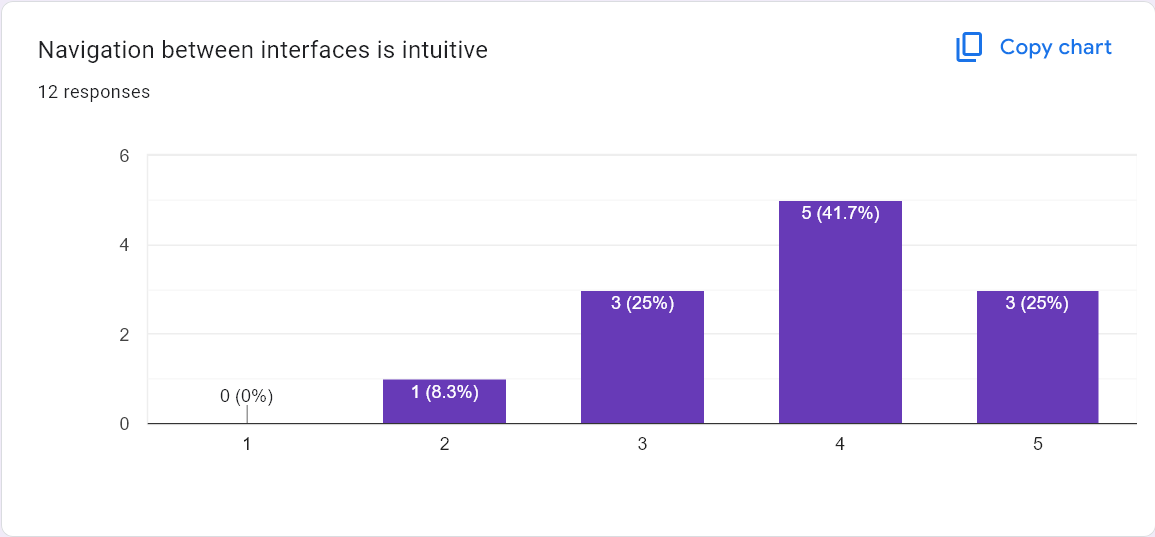
\includegraphics[scale=0.35]{./Images/Q1.png}}
  \label{fig:StraightForward}
\end{figure}

\begin{figure}[htbp]
  \caption{"Placing objects is easy" statement ratings}
  \centerline{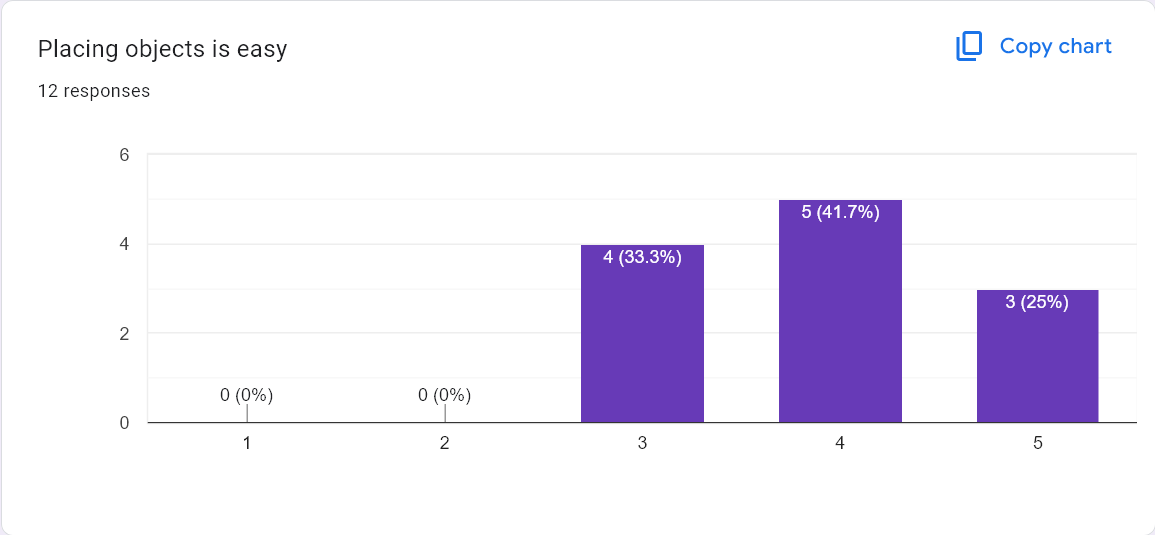
\includegraphics[scale=0.35]{./Images/Q2.png}}
  \label{fig:Navigation}
\end{figure}

\begin{figure}[htbp]
  \caption{"Generating objects is easy" statement ratings}
  \centerline{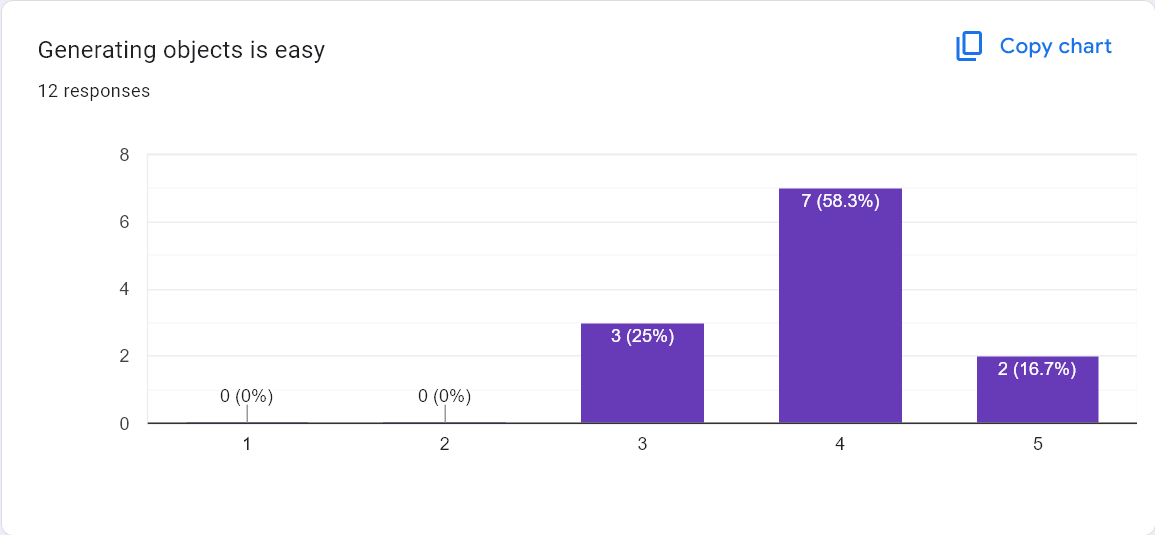
\includegraphics[scale=0.35]{./Images/Q3.png}}
  \label{fig:Detached}
\end{figure}

\begin{figure}[htbp]
  \caption{"It is easy to start a tour" statement ratings}
  \centerline{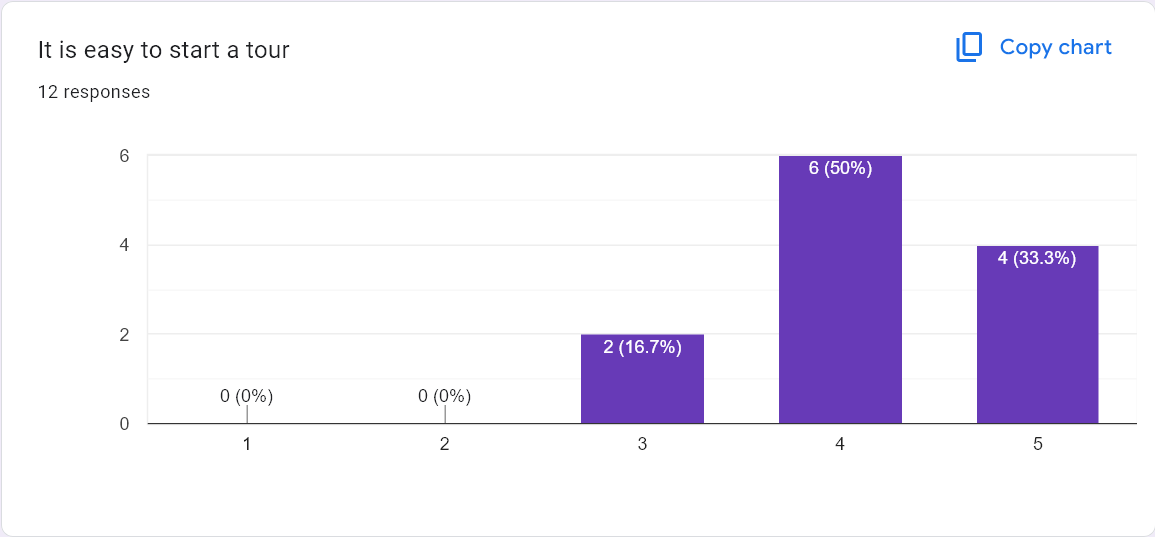
\includegraphics[scale=0.35]{./Images/Q4.png}}
  \label{fig:RealWorld}
\end{figure}

\begin{figure}[htbp]
  \caption{"Changing settings is easy" statement ratings}
  \centerline{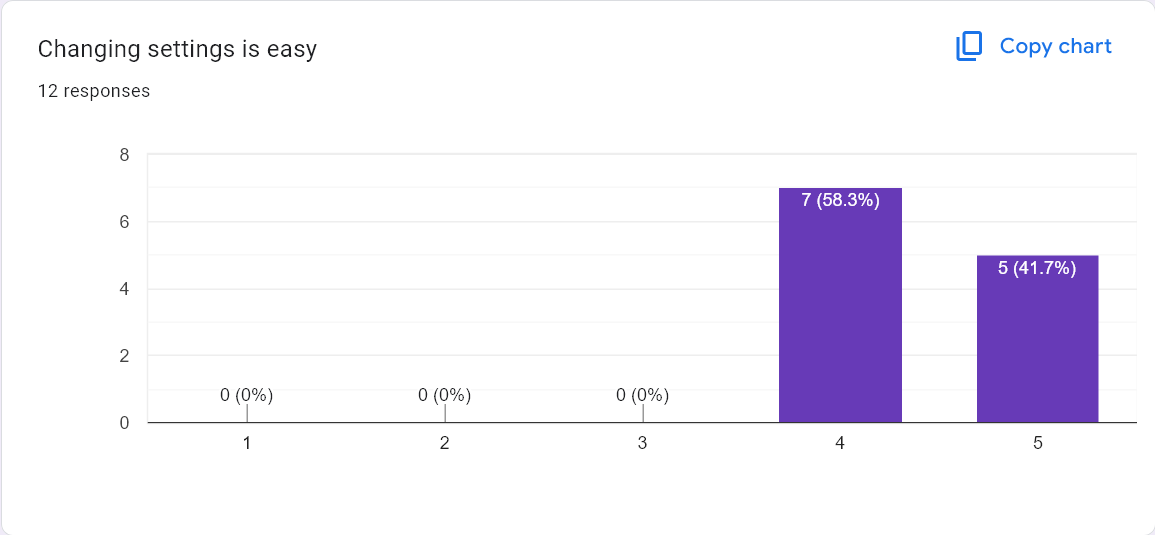
\includegraphics[scale=0.35]{./Images/Q5.png}}
  \label{fig:Fun}
\end{figure}

\begin{figure}[htbp]
  \caption{"The app is generally satisfying to use" statement ratings}
  \centerline{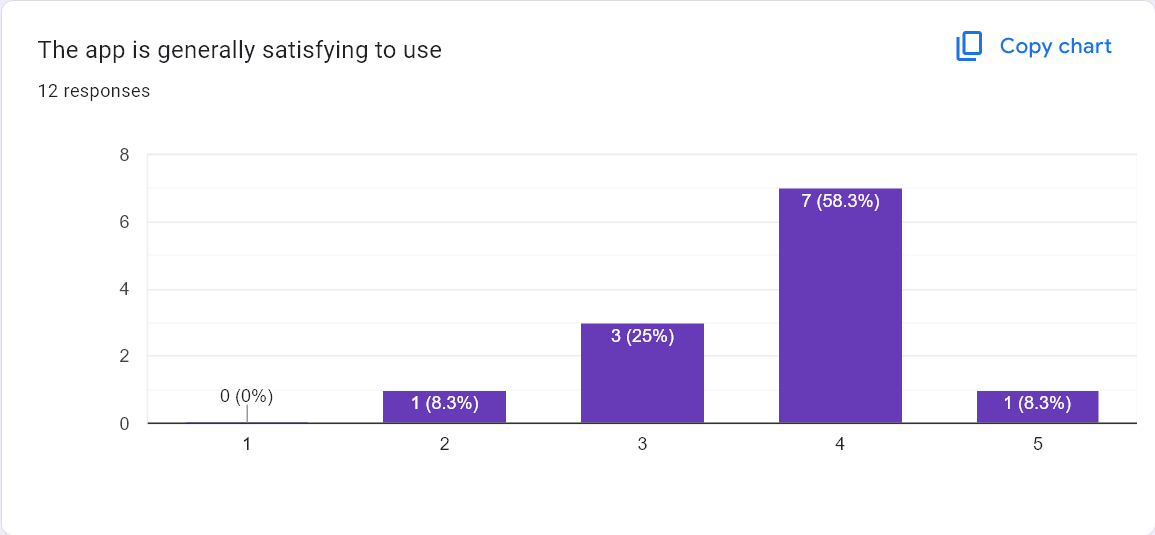
\includegraphics[scale=0.35]{./Images/Q6.png}}
  \label{fig:Social}
\end{figure}

\begin{figure}[htbp]
  \caption{"Using the app distracts from the surroundings" statement ratings}
  \centerline{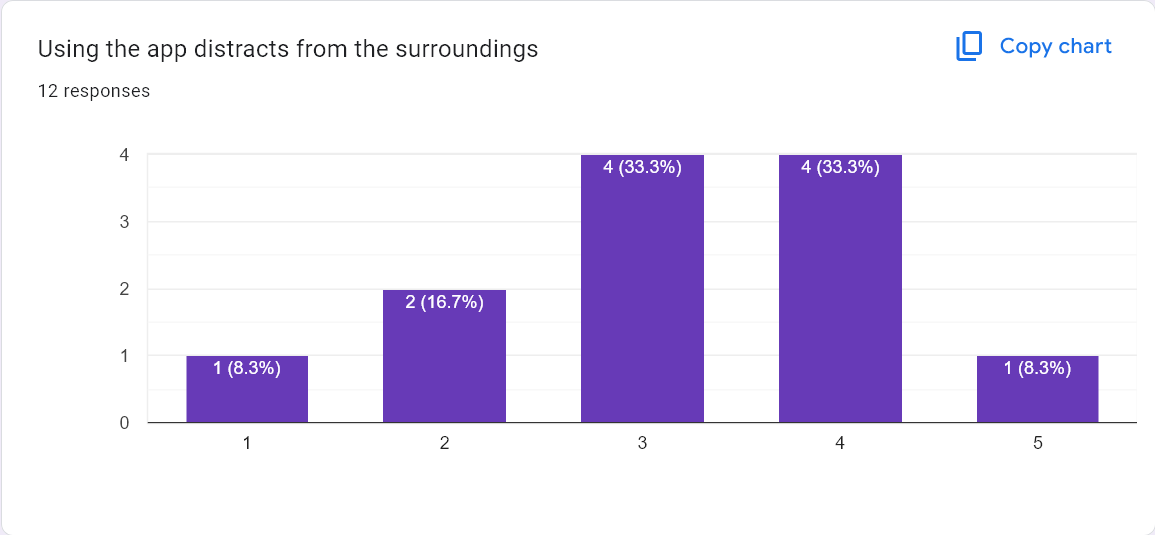
\includegraphics[scale=0.35]{./Images/Q7.png}}
  \label{fig:Enjoy}
\end{figure}

\newpage{}

\section*{Appendix --- Reflection}

The information in this section will be used to evaluate the team members on the
graduate attribute of Reflection.

The purpose of reflection questions is to give you a chance to assess your own
learning and that of your group as a whole, and to find ways to improve in the
future. Reflection is an important part of the learning process.  Reflection is
also an essential component of a successful software development process.  

Reflections are most interesting and useful when they're honest, even if the
stories they tell are imperfect. You will be marked based on your depth of
thought and analysis, and not based on the content of the reflections
themselves. Thus, for full marks we encourage you to answer openly and honestly
and to avoid simply writing ``what you think the evaluator wants to hear.''

Please answer the following questions.  Some questions can be answered on the
team level, but where appropriate, each team member should write their own
response:


\begin{enumerate}
  \item What went well while writing this deliverable?\\ \\
  The unit tests seemed fairly simple and intuitive to do and the work was split up well between the group.
  \item What pain points did you experience during this deliverable, and how
        did you resolve them?\\ \\
    Executing some of the test cases smoothly was a pain point, as well as getting them to pass, but sticking with it and sitting through them after some time, we were able to do our tests and pass them.
  \item Which parts of this document stemmed from speaking to your client(s) or
        a proxy (e.g. your peers)? Which ones were not, and why?\\ \\
        Usability survey and feedback on the app was given from peers. Since we don't have a client, a lot of our feedback was from the Professor and TA during Rev0.
  \item In what ways was the Verification and Validation (VnV) Plan different
        from the activities that were actually conducted for VnV?  If there were
        differences, what changes required the modification in the plan?  Why did
        these changes occur?  Would you be able to anticipate these changes in future
        projects?  If there weren't any differences, how was your team able to clearly
        predict a feasible amount of effort and the right tasks needed to build the
        evidence that demonstrates the required quality?  (It is expected that most
        teams will have had to deviate from their original VnV Plan.)\\ \\
        We had initially expected many of our tests to be automated, but after actually going through them, a lot of them seemed to be more manual work, such as logging in ourselves, testing out the tours, etc. We learned that many of the manual tests are moreso for the code correctness and such, and, at least for our project, the functionality had to be tested through doing.
\end{enumerate}

\end{document}